% Options for packages loaded elsewhere
\PassOptionsToPackage{unicode}{hyperref}
\PassOptionsToPackage{hyphens}{url}
%
\documentclass[
  12pt,
]{article}
\usepackage{lmodern}
\usepackage{amssymb,amsmath}
\usepackage{ifxetex,ifluatex}
\ifnum 0\ifxetex 1\fi\ifluatex 1\fi=0 % if pdftex
  \usepackage[T1]{fontenc}
  \usepackage[utf8]{inputenc}
  \usepackage{textcomp} % provide euro and other symbols
\else % if luatex or xetex
  \usepackage{unicode-math}
  \defaultfontfeatures{Scale=MatchLowercase}
  \defaultfontfeatures[\rmfamily]{Ligatures=TeX,Scale=1}
\fi
% Use upquote if available, for straight quotes in verbatim environments
\IfFileExists{upquote.sty}{\usepackage{upquote}}{}
\IfFileExists{microtype.sty}{% use microtype if available
  \usepackage[]{microtype}
  \UseMicrotypeSet[protrusion]{basicmath} % disable protrusion for tt fonts
}{}
\makeatletter
\@ifundefined{KOMAClassName}{% if non-KOMA class
  \IfFileExists{parskip.sty}{%
    \usepackage{parskip}
  }{% else
    \setlength{\parindent}{0pt}
    \setlength{\parskip}{6pt plus 2pt minus 1pt}}
}{% if KOMA class
  \KOMAoptions{parskip=half}}
\makeatother
\usepackage{xcolor}
\IfFileExists{xurl.sty}{\usepackage{xurl}}{} % add URL line breaks if available
\IfFileExists{bookmark.sty}{\usepackage{bookmark}}{\usepackage{hyperref}}
\hypersetup{
  pdftitle={Turnout and Amendment 4},
  pdfauthor={Kevin Morris},
  hidelinks,
  pdfcreator={LaTeX via pandoc}}
\urlstyle{same} % disable monospaced font for URLs
\usepackage[margin=1in]{geometry}
\usepackage{longtable,booktabs}
% Correct order of tables after \paragraph or \subparagraph
\usepackage{etoolbox}
\makeatletter
\patchcmd\longtable{\par}{\if@noskipsec\mbox{}\fi\par}{}{}
\makeatother
% Allow footnotes in longtable head/foot
\IfFileExists{footnotehyper.sty}{\usepackage{footnotehyper}}{\usepackage{footnote}}
\makesavenoteenv{longtable}
\usepackage{graphicx}
\makeatletter
\def\maxwidth{\ifdim\Gin@nat@width>\linewidth\linewidth\else\Gin@nat@width\fi}
\def\maxheight{\ifdim\Gin@nat@height>\textheight\textheight\else\Gin@nat@height\fi}
\makeatother
% Scale images if necessary, so that they will not overflow the page
% margins by default, and it is still possible to overwrite the defaults
% using explicit options in \includegraphics[width, height, ...]{}
\setkeys{Gin}{width=\maxwidth,height=\maxheight,keepaspectratio}
% Set default figure placement to htbp
\makeatletter
\def\fps@figure{htbp}
\makeatother
\setlength{\emergencystretch}{3em} % prevent overfull lines
\providecommand{\tightlist}{%
  \setlength{\itemsep}{0pt}\setlength{\parskip}{0pt}}
\setcounter{secnumdepth}{5}
\usepackage{rotating}
\usepackage{setspace}\doublespacing
\newcommand{\beginsupplement}{\setcounter{table}{0}  \renewcommand{\thetable}{A\arabic{table}} \setcounter{figure}{0} \renewcommand{\thefigure}{A\arabic{figure}}}
\usepackage{booktabs}
\usepackage{longtable}
\usepackage{array}
\usepackage{multirow}
\usepackage{wrapfig}
\usepackage{float}
\usepackage{colortbl}
\usepackage{pdflscape}
\usepackage{tabu}
\usepackage{threeparttable}
\usepackage{threeparttablex}
\usepackage[normalem]{ulem}
\usepackage{makecell}
\usepackage{xcolor}
\newlength{\cslhangindent}
\setlength{\cslhangindent}{1.5em}
\newenvironment{cslreferences}%
  {\setlength{\parindent}{0pt}%
  \everypar{\setlength{\hangindent}{\cslhangindent}}\ignorespaces}%
  {\par}

\title{Turnout and Amendment 4\thanks{The author thanks Many People for their comments on this project. All errors are my responsibility.}}
\author{Kevin Morris\footnote{Researcher, Brennan Center for Justice at NYU School of Law, 120 Broadway Ste 1750, New York, NY 10271 (\href{mailto:kevin.morris@nyu.edu}{\nolinkurl{kevin.morris@nyu.edu}})}}
\date{February 14, 2020}

\begin{document}
\maketitle
\begin{abstract}
Here is an abstract.
\end{abstract}

\pagenumbering{gobble}
\pagebreak

\pagenumbering{arabic}

\hypertarget{introduction}{%
\section*{Introduction}\label{introduction}}
\addcontentsline{toc}{section}{Introduction}

On November 6\textsuperscript{th}, 2018, Floridians voted to amend their state constitution to allow individuals with felony convictions in their past (Taylor \protect\hyperlink{ref-Taylor2018}{2018}). The move was hailed as transformational for Floridian --- and American --- democracy (Morris \protect\hyperlink{ref-Morris2018}{2018}); the Sentencing Project (\protect\hyperlink{ref-sentencing_2016}{2016}) had estimated a few years earlier that some 1.5 million Floridians were disenfranchised and had finished serving their sentences. The racial implications for the constitutional amendment were also clear: according to the same Sentencing Project report, more than 1 out of every 5 Black Floridians was prohibited from democratic participation thanks to the state's disenfranchisement policies. The Amendment received broad support. Although it needed just 60 percent of the vote to pass, precinct-level data from the Florida Division of Elections shows that 64.5 percent of voters supported the ballot initiative. Conversely, the winning candidates for Governor and United States Senate won just 49.5 and 49.9 percent of the vote, respectively, implying that the constitutional amendment enjoyed some bipartisan support.

Felony disenfranchisement is not unique to Florida's electoral system: in all but two states in the United States, individuals convicted of felony offenses lose their right to vote for at least some period of time (Justice \protect\hyperlink{ref-bcj_laws}{2019}). According to the Brennan Center for Justice, felony convictions result in lifetime prohibitions from voting for some citizens in 11 states based on the severity of the crime.\footnote{Iowa stands alone in disenfranchising all individuals ever convicted of felony offenses.} Nevertheless, the shift in Florida from permanent disenfranchisement for all individuals convicted of felony offenses to restoring voting rights to most individuals\footnote{Individuals convicted of felony sexual assault or murder remain permanently disenfranchised} upon the termination of their sentence moved the needle significantly: according to the same Sentencing Project report, post-sentence Floridians accounted for roughly 24 percent of all disenfranchised Americans (Uggen, Larson, and Shannon \protect\hyperlink{ref-sentencing_2016}{2016}).

The case of Amendment 4 was somewhat unique in how Floridians with felony convictions in their past had their voting rights restored. Usually, the question of voting rights restoration is not put directly to the voters. In New York State in 2018 and Kentucky in 2019, for instance, governors signed executive order restoring voting rights to some disenfranchised individuals (Wang \protect\hyperlink{ref-Wang2018}{2018}; Wines \protect\hyperlink{ref-Wines2019}{2019}). In other states such as Louisiana (Crisp \protect\hyperlink{ref-Crisp2019}{2019}) and Colorado (Baumann \protect\hyperlink{ref-Baumann2019}{2019}), state lawmakers have passed bills restoring voting rights to formerly incarcerated individuals. In Florida, however, put the question was put directly to voters. In the Sunshine State, voters had the opportunity to democratically decide whether they wanted to restore voting rights to their formerly incarcerated or probationed neighbors.

This paper explores whether the presence of Amendment 4 on the ballot increased participation among individuals who live in close proximity to the disenfranchised. There is much literature that establishes that proximal contact with the criminal justice system reduces eligible Americans' propensity to vote (e.g.~Ochs \protect\hyperlink{ref-Ochs2006}{2006}; Bowers and Preuhs \protect\hyperlink{ref-Bowers2009}{2009}; Burch \protect\hyperlink{ref-Burch2013}{2013}; King and Erickson \protect\hyperlink{ref-King2016}{2016}). Little work, however, has been done exploring whether the re-enfranchisement of family and community members can bring back these lost votes. The case of Amendment 4 in Florida offers a unique opportunity to investigate whether these eligible individuals can be reincorporated into our democratic processes.

\hypertarget{theory-and-literature}{%
\section*{Theory and Literature}\label{theory-and-literature}}
\addcontentsline{toc}{section}{Theory and Literature}

\hypertarget{democratic-withdrawal}{%
\subsection*{Democratic Withdrawal}\label{democratic-withdrawal}}
\addcontentsline{toc}{subsection}{Democratic Withdrawal}

\hypertarget{self-interested-voting}{%
\subsection*{Self-Interested Voting}\label{self-interested-voting}}
\addcontentsline{toc}{subsection}{Self-Interested Voting}

\hypertarget{research-design}{%
\section*{Research Design}\label{research-design}}
\addcontentsline{toc}{section}{Research Design}

I begin by testing whether neighborhoods the number of formerly incarcerated individuals living in a neighborhood influenced the turnout in 2018 of that neighborhood. ``Neighborhoods'' and ``turnout'' are defined in multiple ways throughout the neighborhood analysis --- each definition suffers slightly because of data limitations, but together they paint a full picture.

I begin by defining neighborhoods as precincts. Defining neighborhoods as precincts provides two benefits: firstly, because the Florida Division of Elections produces results at this level, we can identify not only how many people cast a ballot at all, but also how many people participated in the contest for Amendment 4. This is an important distinction: voters are more likely to vote for the top-line contests for Governor and United States Senator, and ``roll-off'' (that is, abstain from participating) when it comes to downballot questions such as ballot initiatives {[}CITE{]}. Given that some research indicates that Black voters are more likely to roll-off than white voters (Vanderleeuw and Engstrom \protect\hyperlink{ref-Vanderleeuw1987}{1987}, but see @Knack2008), the question of roll-off is of particular interest when considering a question that intersects with race such as the criminal justice system. Precinct-level data, therefore, allows us to determine not how many voters in a neighborhood voted for \emph{any} contest, but specifically for Amendment 4.

Precinct-level data also allows us to tell the extent to which neighborhoods supported Amendment 4. The secret ballot, of course, prevents us from knowing how individuals voted; precinct-level data, therefore, offer the lowest-level picture of what sorts of communities were more or less likely to support Amendment 4.

Unfortunately, the use of precinct-level data leaves us with a major drawback: when doing analysis at this level, bias-free turnout denominators are hard to come by. Because the Census Bureau does not produce population estimates for individual voting precincts, turnout cannot be calculated by dividing the number of ballots cast by the eligible population; turnout, rather, has to be constructed as a share of registered voters. If there is a relationship between the independent variable of interest and the registration rate of a neighborhood, this could bias our estimates. It is not difficult to imagine how this could be the case in the study at hand. Political organizers working on behalf of Amendment 4's passage may have focused on registering eligible residents neighborhoods where disenfranchised individuals lived, expecting these newly registered voters to support the amendment. If these organizers registered many new voters but a relatively small share of the new voters actually turned out, the net effect might be higher turnout among eligible voters, but \emph{lower} turnout among registered voters.

To address this potential problem, I also define neighborhoods as Census block groups. The Census makes estimates of the citizen voting-age population available at this level, providing a better denominator for calculating turnout. In this case, however, I must use a geocoded voter file to determine turnout. Thus, because I aggregate the number of ballots cast in a block group from individual level data, I am unable to determine whether an individual actually participated in the contest for Amendment 4 or they rolled off. Similarly, I am unable to interrogate the relationship between block group characteristics and support for Amendment 4.

After examining whether the presence of formerly incarcerated individuals was related with a \emph{neighborhood's} turnout rate, I ask whether the individuals with the potentially closest relationship to the disenfranchised voters were more likely to turnout. For this analysis, I use release addresses provided to the DOC and voter file data to identify registered voters who live with formerly incarcerated individuals. Voters are considered ``treated'' if they live with a formerly incarcerated individual, and ``untreated'' otherwise. I then use a variety of individual- and neighborhood-level characteristics to match treated and untreated voters using a genetic algorithm (Sekhon \protect\hyperlink{ref-Sekhon2011}{2011}). After matching these voters, I employ a difference-in-differences specification to determine whether treated voters participated at higher rates in the 2018 election.

\hypertarget{data}{%
\section*{Data}\label{data}}
\addcontentsline{toc}{section}{Data}

I leverage multiple data sources to investigate whether individuals in proximate contact with disenfranchised residents were more likely to vote in the 2018 election.

\hypertarget{department-of-corrections-data}{%
\subsection*{Department of Corrections Data}\label{department-of-corrections-data}}
\addcontentsline{toc}{subsection}{Department of Corrections Data}

Data from the Florida Department of Corrections is used to identify individuals who have been to prison in Florida. These records include all individuals released from prison since October 1, 1997.\footnote{Using the last-known address for individuals last released from prison in 1997 presents some difficulty; it is possible that the formerly incarcerated individuals have died or moved. In Appendix A, I show that the results presented in the body of this article continue to hold even when limiting the pool of formerly incarcerated people to individuals released from prison during or after 2015.} Using records of individuals currently in prison or on parole, I can identify all individuals who had been to prison but were not serving a sentence at the time of the 2018 midterm election. These are the individuals who would be re-enfranchsied by Amendment 4, and therefore the people most likely to encourage their friends and neighbors to vote on their behalf. I include only individuals with a valid release; individuals who died or absconded before their sentence was completed are removed from the dataset. I identify 342,694 such individuals.

The Florida Department of Corrections provides the last-known addresses of all individuals who were formerly incarcerated. The address data, however, are messy. In some cases, the address field is left blank; in others, the records simply notes the road or the town of the former inmate, without providing full address information. These addresses require substantial cleaning.

I begin the cleaning process by removing all records where the address does not begin with an integer. In other words, I assume that any record that begins with a letter does not have a fill address and cannot be used. I then geocode these addresses using Google Maps' geocoder, and drop all individuals whose addresses could not be geocoded or were geocoded outside of Florida. The resulting list includes 286,268. This represents 83.5 percent of the formerly incarcerated individuals. The failure to identify the home location of so many formerly incarcerated individuals may pose problems; if we end up undercounting the number of formerly incarcerated individuals in some neighborhoods, we may underestimate the effects of the presence of formerly incarcerated individuals on neighborhood or individual level turnout.

Many formerly incarcerated individuals leave prison not for homes with family members, but rather to homeless shelters and halfway houses. The body of this paper excludes formerly incarcerated individuals whose last known address was also listed by five or more other individuals, because neighborhoods may respond differently to institutions for returning citizens than the return of a family or community member. Appendix B demonstrates that the primary findings in the paper hold when we include all formerly incarcerated individuals, even if they returned to the same location as many other formerly incarcerated individuals.

The successfully geocoded, formerly incarcerated individuals are then mapped to their home Census block groups using shapefiles from the Census Bureau, and to their home voter precincts using data collected by Kelso and Migurski (\protect\hyperlink{ref-Kelso2018}{2018}).

Statewide data on individuals who formerly served a term on felony probation are not available. This too may pose a problem for this study; neighborhoods with disenfranchised former probationers are also ``treated.'' Such data is available, however from COUNTY COUNTY. In Appendix C, I incorporate these data to interrogate whether the omission of these individuals from the statewide analyses is likely impacting my results.

\hypertarget{voter-file-data}{%
\subsection*{Voter File Data}\label{voter-file-data}}
\addcontentsline{toc}{subsection}{Voter File Data}

Individual-level voter file data are used for a variety of purposes in this analysis. I primarily use Florida voter file data from the data vendor L2. This file includes information on individuals such as their home address, their age and gender, their participation history, and their political affiliation. L2 also geocodes voters to their home Census blocks, and provides latitude and longitudes.

Although the L2 data includes estimates of voters' race and ethnicity, the raw Florida voter file includes self-identificated race and ethnicity. In place of L2's estimates, I use the self-reported data found in the raw Florida voter file (the two lists can be joined using a unique identifier). I also use the raw Florida file to provide the gender for voters for whom L2 did not have an estimate, as well as voters' home counties and precincts.

Precinct and block group demographics are constructed using the voter file data. A precinct's average age, therefore, is the average age of all voters registered in that precinct; the same is true for Census block groups. Some information such as median income, however, is not available at the individual level. For these variables, voters are assigned the median income (or education level, et cetera) of their home block group from the ACS 5 year estimates ending with 2018; the precinct average income, therefore, is effectively the average of all the block groups within that precinct, weighted by the number of registered voters in each block group.

For the individual-level analyses, I use individual-level demographic controls obtained from the voter files, and neighborhood-level demographic controls like income from the voter's block group.

\hypertarget{division-of-election-results-data}{%
\subsection*{Division of Election Results Data}\label{division-of-election-results-data}}
\addcontentsline{toc}{subsection}{Division of Election Results Data}

As discussed above, the Florida Division of Elections makes precinct-level results data available. These data come with precinct identifiers that correspond to the precinct reported in the Florida voter file.

\hypertarget{matched-department-of-corrections-and-voter-file-data}{%
\subsection*{Matched Department of Corrections and Voter File Data}\label{matched-department-of-corrections-and-voter-file-data}}
\addcontentsline{toc}{subsection}{Matched Department of Corrections and Voter File Data}

Identifying eligible registered voters who lived with formerly incarcerated individuals in the 2018 election requires matching on addresses. As discussed above, these addresses are often in different formats. To increase the quality of the matches, I standardize common street and address abbreviations as well as capitalization. ``Boulevard,'' for instance, becomes ``BLVD'' in each instance in the DOC and voter file data. These standardizations are taken from Appendix C of the USPS Postal Addressing Standards (\protect\hyperlink{ref-USPS2015}{2015}). Exact matching is required.

\hypertarget{neighborhood-level-results}{%
\section*{Neighborhood-Level Results}\label{neighborhood-level-results}}
\addcontentsline{toc}{section}{Neighborhood-Level Results}

I begin by examining whether --- and to what extent --- neighborhoods with formerly incarcerated individuals differ from neighborhoods elsewhere in the state. A simple comparison of neighborhoods with and without formerly incarcerated individuals, however, proves unhelpful: 97.4 percent of block groups in the state are home to someone who has been to prison, lending credence to the notion that the criminal justice system impacts nearly every neighborhood in the Sunshine State. There are, however, neighborhoods where formerly incarcerated individuals are concentrated. In Column 1 of Table \ref{tab:demos}, I take the statewide mean of block group characteristics, weighted by each block group's population. In Column 2, I re-weight the block groups by the number of formerly incarcerated residents.

\input{"../temp/table_whatever2.tex"}

Although nearly all parts of the state are impacted by the criminal justice system (and, more specifically, mass incarceration), Table \ref{tab:demos} makes clear that individuals return home to neighborhoods with lower incomes, higher levels of unemployment, and where a much larger share of the population is Black than other neighborhoods.

\hypertarget{precinct-results}{%
\subsection{Precinct Results}\label{precinct-results}}

Having established that formerly incarcerated individuals are concentrated in lower-resourced neighborhoods, I investigate whether turnout in their neighborhoods was higher in 2018 thanks to the inclusion of Amendment 4 on the ballot. To test this relationship I run an OLS regression, where precinct-level turnout is the dependent variable. Turnout is defined by dividing the number of ballots cast for or against Amendment 4 by the number of actively registered voters in the precinct.\footnote{Roughly 0.6 percent of precincts reported turnout of greater than 100 percent; these 35 precincts have been dropped from the analysis.} The number of formerly incarcerated residents\footnote{As discussed above, this includes only formerly incarcerated residents who returned to home addresses reported by three or fewer other formerly incarcerated individuals.} as the primary independent variable.

Table \ref{tab:to-precinct} presents the results of this regression. In addition to the number of formerly incarcerated residents, I control for the racial, gender, and partisan composition of the precinct, as well as turnout rates from the past few elections. Historical turnout is calculated using the registered voter file, not published state results, to account for the redrawing of precinct boundaries between elections. I also control for the average age of the precinct, as well as the median income, share with some collegiate education, and unemployment rate. Finally, fixed effects for congressional districts are included.\footnote{Where precincts cross congressional boundaries, precincts are assigned to the congressional district in which most of their voters live.} Robust standard errors are clustered at the congressional district level.

\begin{singlespace}

\input{"../temp/precinct_to.tex"}
\end{singlespace}

Table \ref{tab:to-precinct} indicates that there is a negative relationship between the number of formerly incarcerated residents in a precinct and the turnout in that precinct among registered voters. The coefficient, however, is small and difficult to interpret. Figure \ref{fig:marg1} shows the marginal effect of each additional disenfranchised resident on precinct-level turnout for Amendment 4. All other covariates are held at their means in this Figure \ref{fig:marg1}. Although the number of disenfranchised residents in a precinct reaches a maximum of 594, there are 300 or fewer disenfranchised residents in 99.2 percent of precincts. Predicted turnout in precincts with zero disenfranchised voters is just over 66 percent; in precincts with 300, predicted turnout was below 61 percent, implying a five point decrease over the effective range of observered values.

\begin{figure}[H]

{\centering 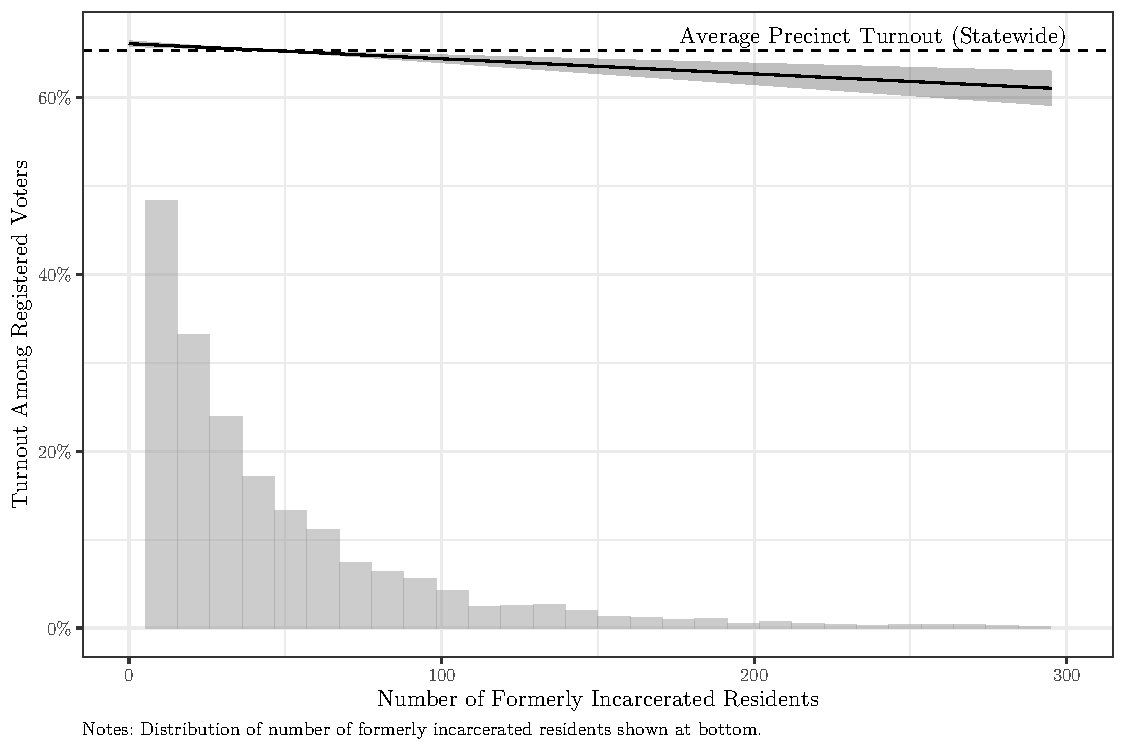
\includegraphics{write_files/figure-latex/marg1-1} 

}

\caption{\label{fig:marg1}Marginal Effect of Each Formerly Incarcerated Residents on Precinct Turnout Among Registered Voters}\label{fig:marg1}
\end{figure}

As discussed above, the use in Table \ref{tab:to-precinct} of registered voters as a denominator for turnout may be muddying what is actually occuring. Voters in the sorts of lower-income neighborhoods home to disproportionate shares of formerly incarcerated individuals are less likely to vote in general {[}CITE{]}. If excitement around Amendment 4 led 10 additional residents of a neighborhood to register, but only 1 of these new registrants actually participated, \emph{overall} turnout was increased even while turnout among registered voters decreased (assuming that the precinct's overall turnout was, in this case, above 10 percent).

To test whether this in fact happened, I begin by examining registrations increased more quickly in the run-up to the 2018 election in neighborhoods with more formerly incarcerated individuals. Using registration dates obtained from the registered voter file, I calculate the number of monthly registrations in each precinct in the state between January 1, 2010, and October 31, 2018. Although the effort to collect signatures to get Amendment 4 on the ballot took place over the course of years, the intiative officially received enough ballots on January 23\textsuperscript{rd}, 2018 (Bousquet \protect\hyperlink{ref-Bousquet2018}{2018}). I therefore use February, 2018, through October, 2018, as the ``treatment'' period. If registrations increased more quickly during this period in places with more formerly incarcerated individuals, this could explain the low turnout observed among registered voters in these neighborhoods.

Table \ref{tab:neg-bin} presents the results of a regression testing whether this in fact occured. Because monthly registrations are counts, a standard OLS regression is inappropriate. Because tests indicate that overdispersion may be present in the data, I fit the model using a negative binomial specification. A dummy indicating the treatment months is indicated with the number of formerly incarcerated precinct residents. The same precinct-level controls are used as in Table \ref{tab:to-precinct}, with the inclusion of a time trend variable.

\begin{singlespace}

\input{"../temp/table_neg_binom.tex"}
\end{singlespace}

The coefficient on D(February -- October, 2018) in Table \ref{tab:neg-bin} indicates monthly registrations were higher across the state in 2018 than in previous years. Although this is perhaps in part due to Amendment 4, the 2018 midterm elections saw higher turnout than any midterm in over a century {[}CITE{]}; there would likely have been a spike in registrations even in the absense of Amendment 4, given the competitive nature of the gubernatorial and United States senate races on the ballot in Florida that year.

Table \ref{tab:neg-bin} also indicates that, over the whole period, monthly registrations were higher in precincts with more formerly incarcerated individuals. We cannot reject the null hypothesis, however, that Amendment 4 did not lead to more registrations in 2018 in neighborhoods with more formerly incarcerated residents. In other words, although registrations did increase over this period in communities with formerly incarcerated residents, this increase was not statistically distinguishable from the increase in registrations in other parts of the state. The depressed turnout in these neighborhoods in 2018, therefore, probably cannot be attributed to higher registration rates among voters with a lower propensity to vote.

Although the precinct-level model implies that \emph{turnout} for Amendment 4 was lower in the places most directly impacted by disenfranchisement laws, the precinct-level data allows us to test for other relationships between the number of formerly incarcerated residents in a neighborhood and that neighborhood's engagement with Amendment 4. In Table \ref{tab:other-precincts} I present the results of OLS models that test whether the number of formerly incarcerated community members influences a neighborhood's support for Amendment 4, and Amendment 4 roll-off. Roll-off is calculated as \(1 - \frac{Ballots\:Cast\:for\:Amendment\:4}{Ballots\:Cast\:in\:Contest\:with\:the\:Most\:Votes}\). It ranges from zero (if everyone who cast a ballot made a decision on the Amendment 4 question) to one (if no participants voted for or against Amendment 4).

\begin{singlespace}

\input{"../temp/precinct_other.tex"}
\end{singlespace}

Table \ref{tab:other-precincts} demonstrates that, although Amendment 4 does not appear to have boosted precinct-level turnout relative to other precincts' turnout, precincts with more formerly incarcerated residents \emph{did} support Amendment 4 at slightly higher rates. Similarly, roll-off was lower in these neighborhoods, which means that a higher share of residents expressed a preference on the question. Thus it appears that the presence of formerly incarcerated individuals in a neighborhood was not associated with getting people into the polling place, it was associated with how voters who \emph{did} participate cast their ballots.

\hypertarget{block-group-results}{%
\subsection*{Block Group Results}\label{block-group-results}}
\addcontentsline{toc}{subsection}{Block Group Results}

As a final test of the relationship between the presence of formerly incarcerated community members, Amendment 4, and turnout in 2018, I use turnout at the Census block group level. As discussed above, the Census Bureau provides estimates of the citizen voting age population (or CVAP) in each block group, which provides a denominator which is unbiased by uneven registration rates. In the block group analysis, I subtract the number of formerly incarcerated residents from the CVAP, because they were ineligible to participate in the election. The number of votes cast in a block group come aggregating the individual voter file; turnout is calculated by dividing the number of voters who participated by the adjusted CVAP estimates.

Table \ref{tab:to-bg} fits the same suite of covariates from Table \ref{tab:to-precinct} on the block group level data. In this block group model, racial characteristics are taken from the ACS 5 year estimates ending in 2018, rather than from the registered voters in that block group. As before, robust standard errors are clustered by congressional district.

\begin{singlespace}

\input{"../temp/bg_to.tex"}
\end{singlespace}

Table \ref{tab:to-bg} demonstrates that, even when turnout is calculated as the share of adjusted CVAP, neighborhoods with more formerly incarcerated residents turned out at lower rates. The effect in this model, however, is smaller than in the precinct-model: the predicted turnout in a block group with no formerly incarcerated residents was 54.8 percent, when all other are set to their means; in block groups with 115 formerly incarcerated residents (the 99 percent bound) the predicted turnout was 53.0 percent, implying a decrease of fewer than 2 percentage points over the effective range of the observed data. Although this estimation of turnout uncovers smaller negative effects than the precinct-based model, it still appears that the presence of Amendment 4 on the ballot in the 2018 did not boost turnout for directly impacted communities by enough to overcome the negative depressive effects of criminal justice involvement.

\hypertarget{individual-level-results}{%
\section*{Individual-Level Results}\label{individual-level-results}}
\addcontentsline{toc}{section}{Individual-Level Results}

Thus far I have established that neighborhoods with more formerly incarcerated residents turned out at lower rates than other neighborhoods. Although this is in line with past scholarship that has found negative indirect turnout effects from incarceration and felony disenfranchisement, it is sobering to note that even a ballot initiative that would increase these neighborhoods' political representation via the expansion of the franchise was not enough to overcome these negative effects.

The use of neighborhood data, however, can obscure underlying patterns. The use of administrative data, as Walker (\protect\hyperlink{ref-Walker2020}{2020}) puts it, does ``not accurately assess the relational aspect central to the concept of proximal contact'' (123). The finding that neighborhood turnout is lower in places with more formerly incarcerated individuals does not help us understand the mechanism(s) through which proximal contact causes lower turnout.

An examination of the relationship between individual-level proximal contact and turnout does not entirely obviate the problem described by Walker (\protect\hyperlink{ref-Walker2020}{2020}) and others. If turnout is lower among the eligible household members of a formerly incarcerated individual, we cannot immediately attribute that decrease to perceptions of injusice. We can imagine other causal mechanisms through which cohabitating with a formerly incarcerated person would reduce propensity to vote. Re-integrating citizens may, for example, have a hard time finding employment; household members may therefore be required to work more hours, reducing their capacity to engage in political information gathering and participation. {[}CITATIONS{]}

Nevertheless, examining the relationship between cohabitation with formerly incarcerated individuals and turnout can shed light on the ways in which proximal contact depress turnout. It is possible that Amendment 4 shaped turnout differently for individuals who cohabitate with formerly incarcerated individuals than for their neighbors. A neighborhood may have disengaged from the political process thanks to a history of aggressive state action. Household members of the formerly incarcerated may have had a similar historical response, and yet be more susceptible to mobilization from Amendment 4's placement on the ballot; their family members and housemates, after all, are the individuals who stood to benefit from the passage of the Amendment. These formerly incarcerated individuals may have successfully mobilized other members of their households but failed to do so for their neighborhood.

Using individual-level data, I here distinguish the effect of proximal neighborhood contact from individual-level contact on turnout in 2018. As discussed above, I identify individuals who live with formerly incarcerated individuals by matching addresses listed in the Department of Corrections release data to the registered voter file. All registered voters who live at an address reported by a formerly incarcerated individual are considered ``treated'' with proximal contact to the carceral state.

Each treated individual is then matched with five untreated registered voters elsewhere in the state.\footnote{Due to computing constraints, a random 1 percent random sample stratified by treatment status is used to calculate the genetic weights. The full sample is used for matching.} Exact matching is done on all characteristics with the exception of registration date, age, median income, and share with some collegiate education, and matching is done with replacement. Voters are matched using their block group's median income and share with some collegiate education (from the ACS 5 year estimates ending in 2018), while all other characteristics come from the individual-level voter file. Table \ref{tab:bal-table} presents the results of this matching exercise.

\begin{table}[H]

\caption{\label{tab:balance-tab-chunk}\label{tab:bal-table} Balance Table}
\centering
\resizebox{\linewidth}{!}{
\begin{tabular}[t]{lllllrrrr}
\toprule
\multicolumn{1}{c}{ } & \multicolumn{2}{c}{Means: Unmatched Data} & \multicolumn{2}{c}{Means: Matched Data} & \multicolumn{4}{c}{Percent Improvement} \\
\cmidrule(l{3pt}r{3pt}){2-3} \cmidrule(l{3pt}r{3pt}){4-5} \cmidrule(l{3pt}r{3pt}){6-9}
 & Treated & Control & Treated & Control & Mean Diff & eQQ Med & eQQ Mean & eQQ Max\\
\midrule
\%White & 41.0\% & 63.0\% & 41.0\% & 41.0\% & 100.00 & 100.00 & 100.00 & 100.00\\
\% Black & 39.0\% & 13.0\% & 39.0\% & 39.0\% & 100.00 & 100.00 & 100.00 & 100.00\\
\% Latino & 13.0\% & 17.0\% & 13.0\% & 13.0\% & 100.00 & 100.00 & 100.00 & 100.00\\
\% Asian & 1.0\% & 2.0\% & 1.0\% & 1.0\% & 100.00 & 100.00 & 100.00 & 100.00\\
\% Female & 55.0\% & 52.0\% & 55.0\% & 55.0\% & 100.00 & 100.00 & 100.00 & 100.00\\
\% Male & 41.0\% & 45.0\% & 41.0\% & 41.0\% & 100.00 & 100.00 & 100.00 & 100.00\\
Registration Date & 2004-02-17 & 2004-09-23 & 2004-02-17 & 2004-02-20 & 98.40 & 93.90 & 85.57 & 64.79\\
Age & 48.87 & 52.45 & 48.87 & 48.85 & 99.35 & 99.37 & 99.23 & 98.81\\
\% Democrat & 54.0\% & 37.0\% & 54.0\% & 54.0\% & 100.00 & 100.00 & 100.00 & 100.00\\
\% Republican & 21.0\% & 35.0\% & 21.0\% & 21.0\% & 100.00 & 100.00 & 100.00 & 100.00\\
\% with Some College & 67.0\% & 75.0\% & 67.0\% & 67.0\% & 99.92 & 99.88 & 99.82 & 99.42\\
Median Income & \$47,481 & \$62,998 & \$47,481 & \$47,503 & 99.86 & 99.78 & 99.60 & 98.46\\
\bottomrule
\end{tabular}}
\end{table}

As Table \ref{tab:bal-table} makes clear, the treated registered voters differ in meaningful ways from the rest of the electorate: they are three times as likely to be Black, they are substantially more likely to be registered as Democrats, and they live in neighborhoods with lower incomes. The matching process, however, results in a control group that is very similar to the treatment group; in each measure, there was at least a 98 percent improvement in the mean difference.

After matching the treated voters to appropriate controls, I construct a difference-in-differences model. Before presenting the results of the model, I show in Figure \ref{fig:dind} that the parallel trends assumption is satisfied: although the treatment group has lower turnout rates in general, the distance between the treatment and control groups is largely constant between 2010 and 2016.

\begin{figure}[H]

{\centering 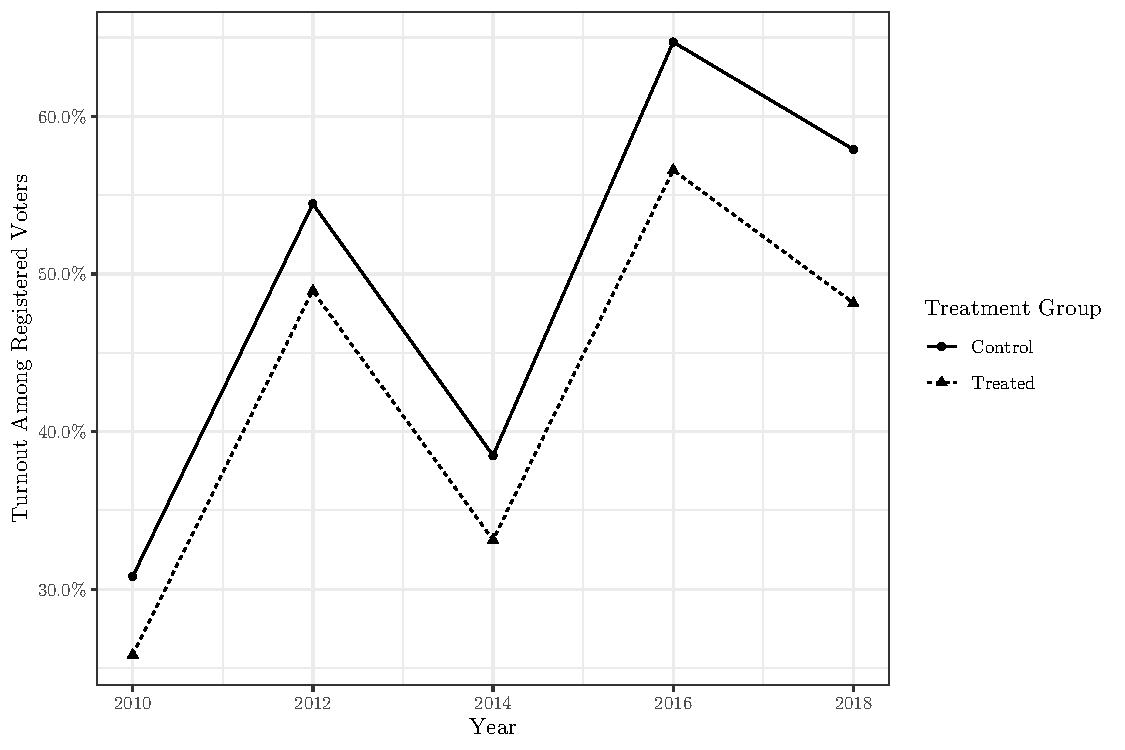
\includegraphics{write_files/figure-latex/dind-1} 

}

\caption{\label{fig:dind}General Election Turnout for Treated and Control Voters, 2010 -- 2018}\label{fig:dind}
\end{figure}

The trends presented in Figure \ref{fig:dind} offer preliminary corroboration of what I find at the neighborhood level --- namely, that proximal contact with formerly incarcerated individuals resulted in lower, not higher, turnout in the 2018 election even after controlling for (here, individual-level) historical turnout. Table \ref{tab:tab-dind} formalizes these trends into a logistic regression. The dependent variable takes the value 0 if the voter did not vote, and 1 if she did. A treatment dummy distinguishes treated from control voters. The treatment dummy is interacted with another dummy identifying the 2018 election. Robust standard errors are clustered at the level of the match (Abadie and Spiess \protect\hyperlink{ref-Abadie2019}{2019}), and each control observation is assigned one-fifth the weight of the treatment observations (to account for the five-to-one match). Model 1 presents the model output without the other controls used for matching; Model two includes these covariates.

In Models 3 and 4 of Table \ref{tab:tab-dind} I consider the possibility that, as households become further removed from a member's incarceration, the negative effects of their incarceration on turnout dissipate. In these models, the dummies indicating treatment and the 2018 election are interacted with the number of years since the most recent completion of a term of incarceration for a household member. Matched control observations are assigned the value associated with their treated observation. Model 3 includes no other covariates, while Model 4 includes the matched variables.

It is, of course, highly possible that formerly incarcerated individuals no longer live in the same household they reported when leaving prison; this is especially true for individuals released from prison early in the sample. To control for this possibility, Models 5 -- 8 include only the treated individuals (and their matches) whose registration dates are earlier than the latest prison release date of a household member. These are individuals, therefore, that we can be sure lived with an incarcerated individual.

\begin{singlespace}
\input{"../temp/dind_reg.tex"}
\end{singlespace}

In each of the specifications presented in Table \ref{tab:tab-dind}, treated individuals were less likely to vote in 2018 after controlling for both their own vote history and the vote history of their matched counterparts. The models that incorporate information about how long their housemates had been out of prison indicate, however, that this effect is moderated by time: individuals who lived with housemates who had not been imprisoned in many years were more likely to vote in 2018 than other voters.

That the effect is moderated by time is unsurprising. Individuals whose household members went to and were released from prison between the 2016 and 2018 elections, for instance, received two treatments: they both were ``negatively'' treated by their proximal contact with the criminal justice system and potentially ``positively'' treated by the presence of Amendment 4. What \emph{is} surprising, however, is that D(2018) is still associated with a negative treatment even for the households that were most removed from their proximal contact with the incarceration of a household member. Table \ref{tab:oldies} presents the results of Models 5 and 6 from Table \ref{tab:tab-dind}, but limits the pool to households where the most recent incarceration ended prior to 2010. This pool is restricted to individuals we are certain lived with formerly incarcerated individuals, and the negative shock of proximal contact for these individuals should be reflected in the base years of the difference-in-differences models. That D(2018) remains significant and negative for these individuals is puzzling.

\begin{singlespace}
\input{"../temp/dind_reg_medium.tex"}
\end{singlespace}

\newpage

\hypertarget{references}{%
\section*{References}\label{references}}
\addcontentsline{toc}{section}{References}

\hypertarget{refs}{}
\begin{cslreferences}
\leavevmode\hypertarget{ref-Abadie2019}{}%
Abadie, Alberto, and Jann Spiess. 2019. ``Robust Post-Matching Inference.'' \emph{Working Paper.}

\leavevmode\hypertarget{ref-Baumann2019}{}%
Baumann, Joella. 2019. ``Paroled Coloradans Are Now Eligible to Vote.'' \emph{Colorado Public Radio}, July 1, 2019. \url{https://www.cpr.org/2019/07/01/paroled-coloradans-are-now-eligible-to-vote/}.

\leavevmode\hypertarget{ref-Bousquet2018}{}%
Bousquet, Steve. 2018. ``Florida Voters Will Have Say on Restoring Voting Rights to Felons.'' \emph{Tampa Bay Times: Florida Politics}, January 23, 2018. \url{https://www.tampabay.com/florida-politics/buzz/2018/01/23/florida-voters-will-have-say-on-restoring-voting-rights-to-felons/}.

\leavevmode\hypertarget{ref-Bowers2009}{}%
Bowers, Melanie, and Robert R. Preuhs. 2009. ``Collateral Consequences of a Collateral Penalty: The Negative Effect of Felon Disenfranchisement Laws on the Political Participation of Nonfelons*.'' \emph{Social Science Quarterly} 90 (3): 722--43. \url{https://doi.org/10.1111/j.1540-6237.2009.00640.x}.

\leavevmode\hypertarget{ref-Burch2013}{}%
Burch, Traci R. 2013. ``Effects of Imprisonment and Community Supervision on Neighborhood Political Participation in North Carolina:'' \emph{The ANNALS of the American Academy of Political and Social Science}, November. \url{https://doi.org/10.1177/0002716213503093}.

\leavevmode\hypertarget{ref-Crisp2019}{}%
Crisp, Elizabeth. 2019. ``Thousands of Felons in Louisiana Will Regain Voting Rights When This Law Takes Effect March 1.'' \emph{The Advocate}, February 15, 2019. \url{https://www.theadvocate.com/baton_rouge/news/politics/article_8a73810c-3153-11e9-81bd-97a9537e8c8b.html}.

\leavevmode\hypertarget{ref-bcj_laws}{}%
Justice, Brennan Center for. 2019. ``Criminal Disenfranchisement Laws Across the United States.'' May 30, 2019. \url{https://www.brennancenter.org/our-work/research-reports/criminal-disenfranchisement-laws-across-united-states}.

\leavevmode\hypertarget{ref-Kelso2018}{}%
Kelso, Nathaniel, and Michael Migurski. 2018. ``Election-Geodata.'' 2018. \url{https://github.com/nvkelso/election-geodata}.

\leavevmode\hypertarget{ref-King2016}{}%
King, Bridgett A., and Laura Erickson. 2016. ``Disenfranchising the Enfranchised: Exploring the Relationship Between Felony Disenfranchisement and African American Voter Turnout.'' \emph{Journal of Black Studies}, July. \url{https://doi.org/10.1177/0021934716659195}.

\leavevmode\hypertarget{ref-Knack2008}{}%
Knack, Stephen, and Martha Kropf. 2008. ``Roll-Off at the Top of the Ballot: International Undervoting in American Presidential Elections.'' \emph{Politics \& Policy} 31 (4): 575--94. \url{https://doi.org/10.1111/j.1747-1346.2003.tb00163.x}.

\leavevmode\hypertarget{ref-Morris2018}{}%
Morris, Kevin. 2018. ``A Transformative Step for Democracy in Florida.'' Brennan Center for Justice. November 7, 2018. \url{https://www.brennancenter.org/our-work/analysis-opinion/transformative-step-democracy-florida}.

\leavevmode\hypertarget{ref-Ochs2006}{}%
Ochs, Holona Leanne. 2006. ``\,`Colorblind' Policy in Black and White: Racial Consequences of Disenfranchisement Policy.'' \emph{Policy Studies Journal} 34 (1): 81--93. \url{https://doi.org/10.1111/j.1541-0072.2006.00146.x}.

\leavevmode\hypertarget{ref-Sekhon2011}{}%
Sekhon, Jasjeet S. 2011. ``Multivariate and Propensity Score Matching Software with Automated Balance Optimization: The Matching Package for R.'' \emph{Journal of Statistical Software} 42 (1): 1--52. \url{https://doi.org/10.18637/jss.v042.i07}.

\leavevmode\hypertarget{ref-Taylor2018}{}%
Taylor, Adam. 2018. ``Florida's Move to Allow Ex-Felons to Vote Brings U.S. Closer to International Election Norms.'' \emph{Washington Post: WorldViews}, November 7, 2018. \url{https://www.washingtonpost.com/world/2018/11/07/floridas-move-allow-ex-felons-vote-brings-us-closer-international-election-norms/}.

\leavevmode\hypertarget{ref-sentencing_2016}{}%
Uggen, Christopher, Ryan Larson, and Sarah Shannon. 2016. ``6 Million Lost Voters: State-Level Estimates of Felony Disenfranchisement, 2016.'' Research report. The Sentencing Project. \url{https://www.sentencingproject.org/publications/6-million-lost-voters-state-level-estimates-felony-disenfranchisement-2016/}.

\leavevmode\hypertarget{ref-USPS2015}{}%
USPS. 2015. ``Appendix C.'' Postal Addressing Standards. May 2015. \url{https://pe.usps.com/text/pub28/28apc_002.htm}.

\leavevmode\hypertarget{ref-Vanderleeuw1987}{}%
Vanderleeuw, James M., and Richard L. Engstrom. 1987. ``Race, Referendums, and Roll-Off.'' \emph{The Journal of Politics} 49 (4): 1081--92. \url{https://doi.org/10.2307/2130785}.

\leavevmode\hypertarget{ref-Walker2020}{}%
Walker, Hannah L. 2020. ``Targeted: The Mobilizing Effect of Perceptions of Unfair Policing Practices.'' \emph{The Journal of Politics} 82 (1): 119--34. \url{https://doi.org/10.1086/705684}.

\leavevmode\hypertarget{ref-Wang2018}{}%
Wang, Vivian. 2018. ``Cuomo Plans to Restore Voting Rights to Paroled Felons.'' \emph{The New York Times: New York}, April 18, 2018. \url{https://www.nytimes.com/2018/04/18/nyregion/felons-pardon-voting-rights-cuomo.html}.

\leavevmode\hypertarget{ref-Wines2019}{}%
Wines, Michael. 2019. ``Kentucky Gives Voting Rights to Some 140,000 Former Felons.'' \emph{The New York Times: U.S.}, December 12, 2019. \url{https://www.nytimes.com/2019/12/12/us/kentucky-felons-voting-rights.html}.
\end{cslreferences}

\end{document}
